\section{Measurement Procedures}
Measurement procedures include preparing samples, preparing the spectrometer, preparing parameters and sample list files for routine measurement, cleanup, and shutting down.

%\subsection{Sample preparation}
%Sample collection will be covered by the separate quality assurance plan. This QAPP covers only the measurement of filter samples.

%When the air filter samples are loaded into the sample holder in the FT-IR spectrometer in Step 8 of Section 8.3 ``Taking a routine measurement," the air filter should be oriented ... %%%%% The sample holder can best be described with a photo, but the sample holder design is proprietary and patent pending. Since this is no longer an SOP and is now a QAPP, this QAPP will not describe the step-by-step process of using the sample holder.

\subsection{Preparing the spectrometer for measurement}
\begin{enumerate}
    \item Make sure the Bruker TENSOR II FT-IR spectrometer (Figure \ref{FTIRphoto}) has been on for at least two hours.
    \item If the TENSOR II FT-IR is off, turn it on using the switch in the back, indicated in Figure \ref{FTIRswitch}. Wait two hours.
\begin{figure}[htp]
\begin{center}
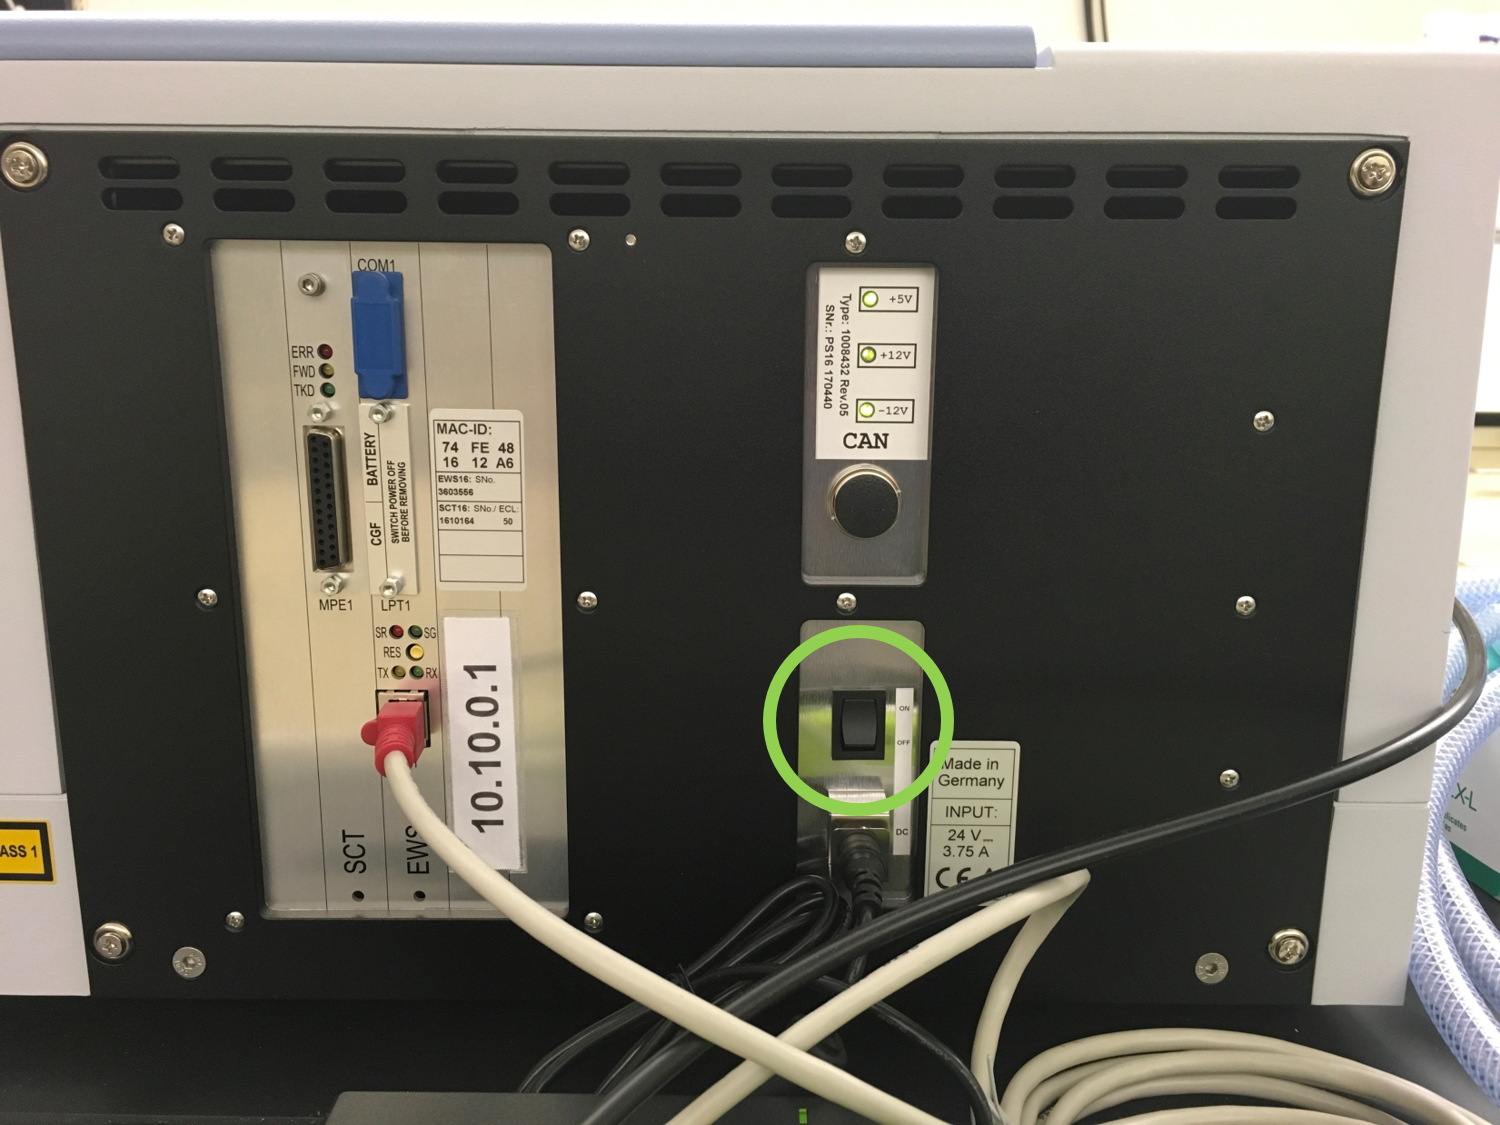
\includegraphics[width=6.5in]{onoffswitchcircle.png}
\caption{Back of the TENSOR II FT-IR, with the on/off switch indicated in a green circle.}
\label{FTIRswitch}
\end{center}
\end{figure}

    \item Fill the liquid nitrogen dewar on the MCT detector (Figure \ref{N2l}). Follow the TENSOR II User Manual Section 5.10, ``Cooling the MCT Detector." It takes approximately 0.5 L of liquid nitrogen to fill the detector dewar. After filling the dewar, wait 5 minutes for the detector temperature to stabilize. A full liquid nitrogen dewar on the MCT detector will hold at operating temperature for 8 hours.
\begin{figure}[htp]
\begin{center}
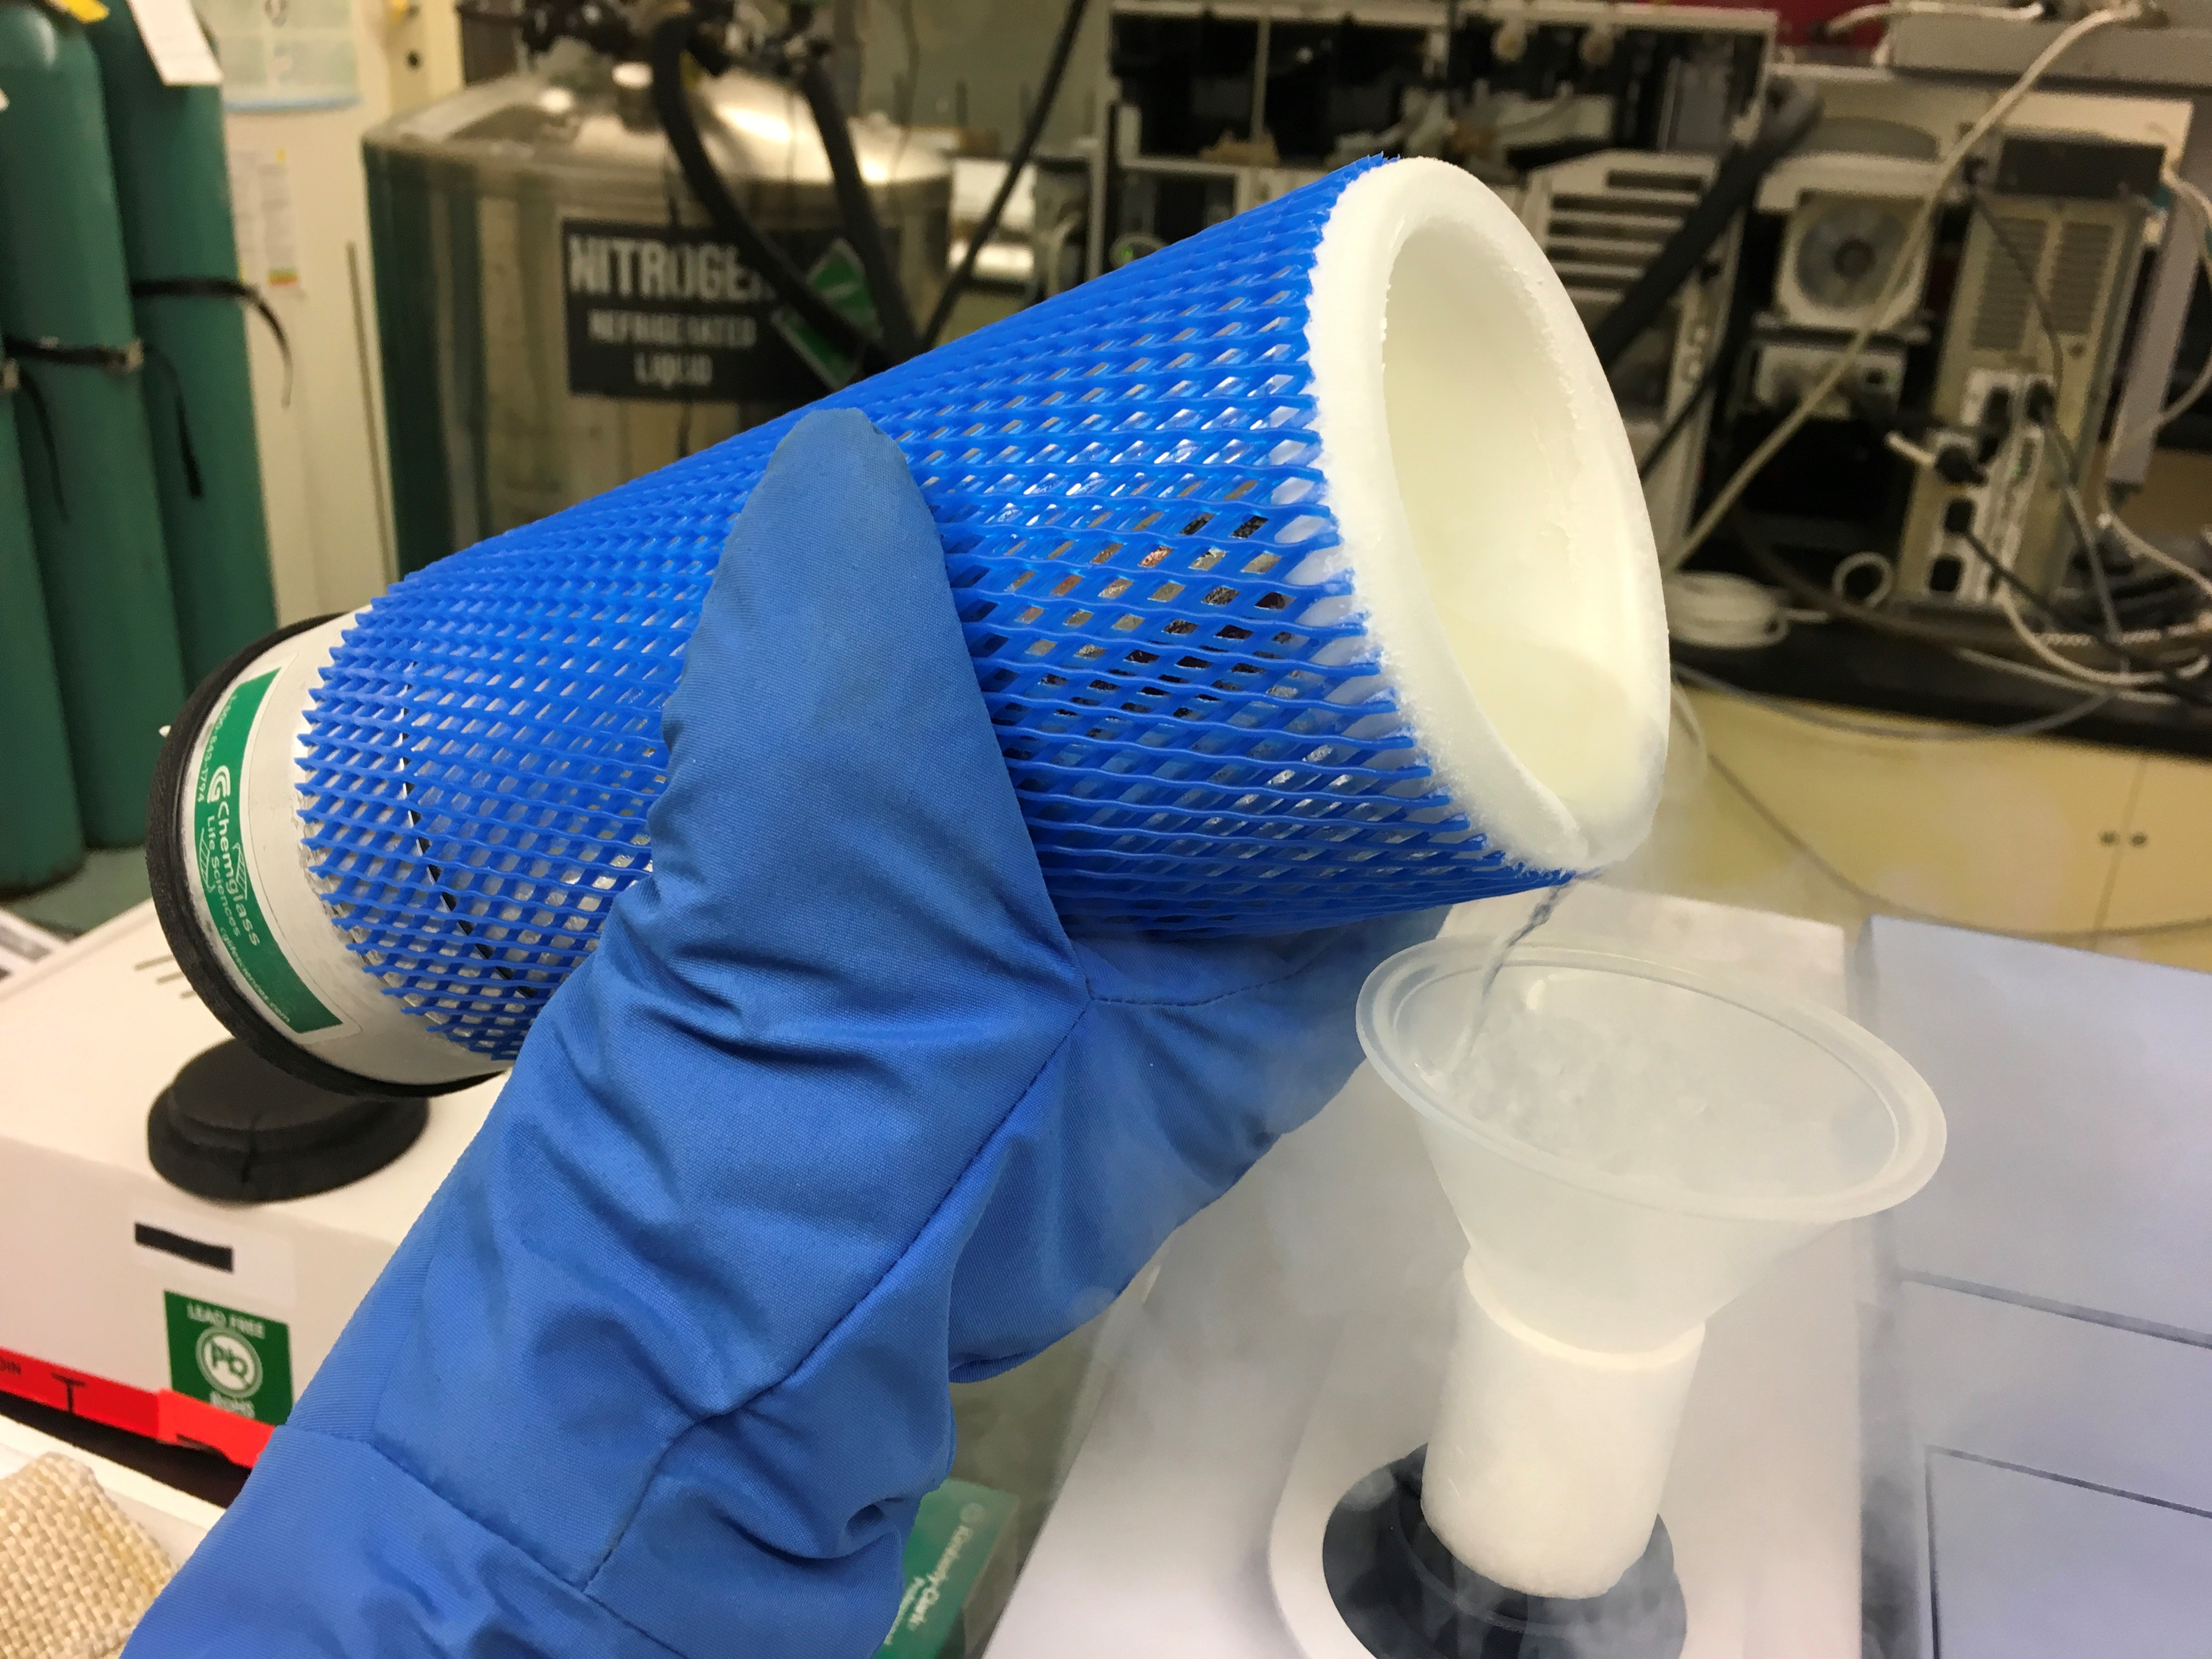
\includegraphics[width=6.5in]{pourN2.jpg}
\caption{Liquid nitrogen pouring.}
\label{N2l}
\end{center}
\end{figure}

    \item Double click the OPUS software icon on the desktop (see Figure \ref{desktopicon}).
\begin{figure}[htp]
\begin{center}
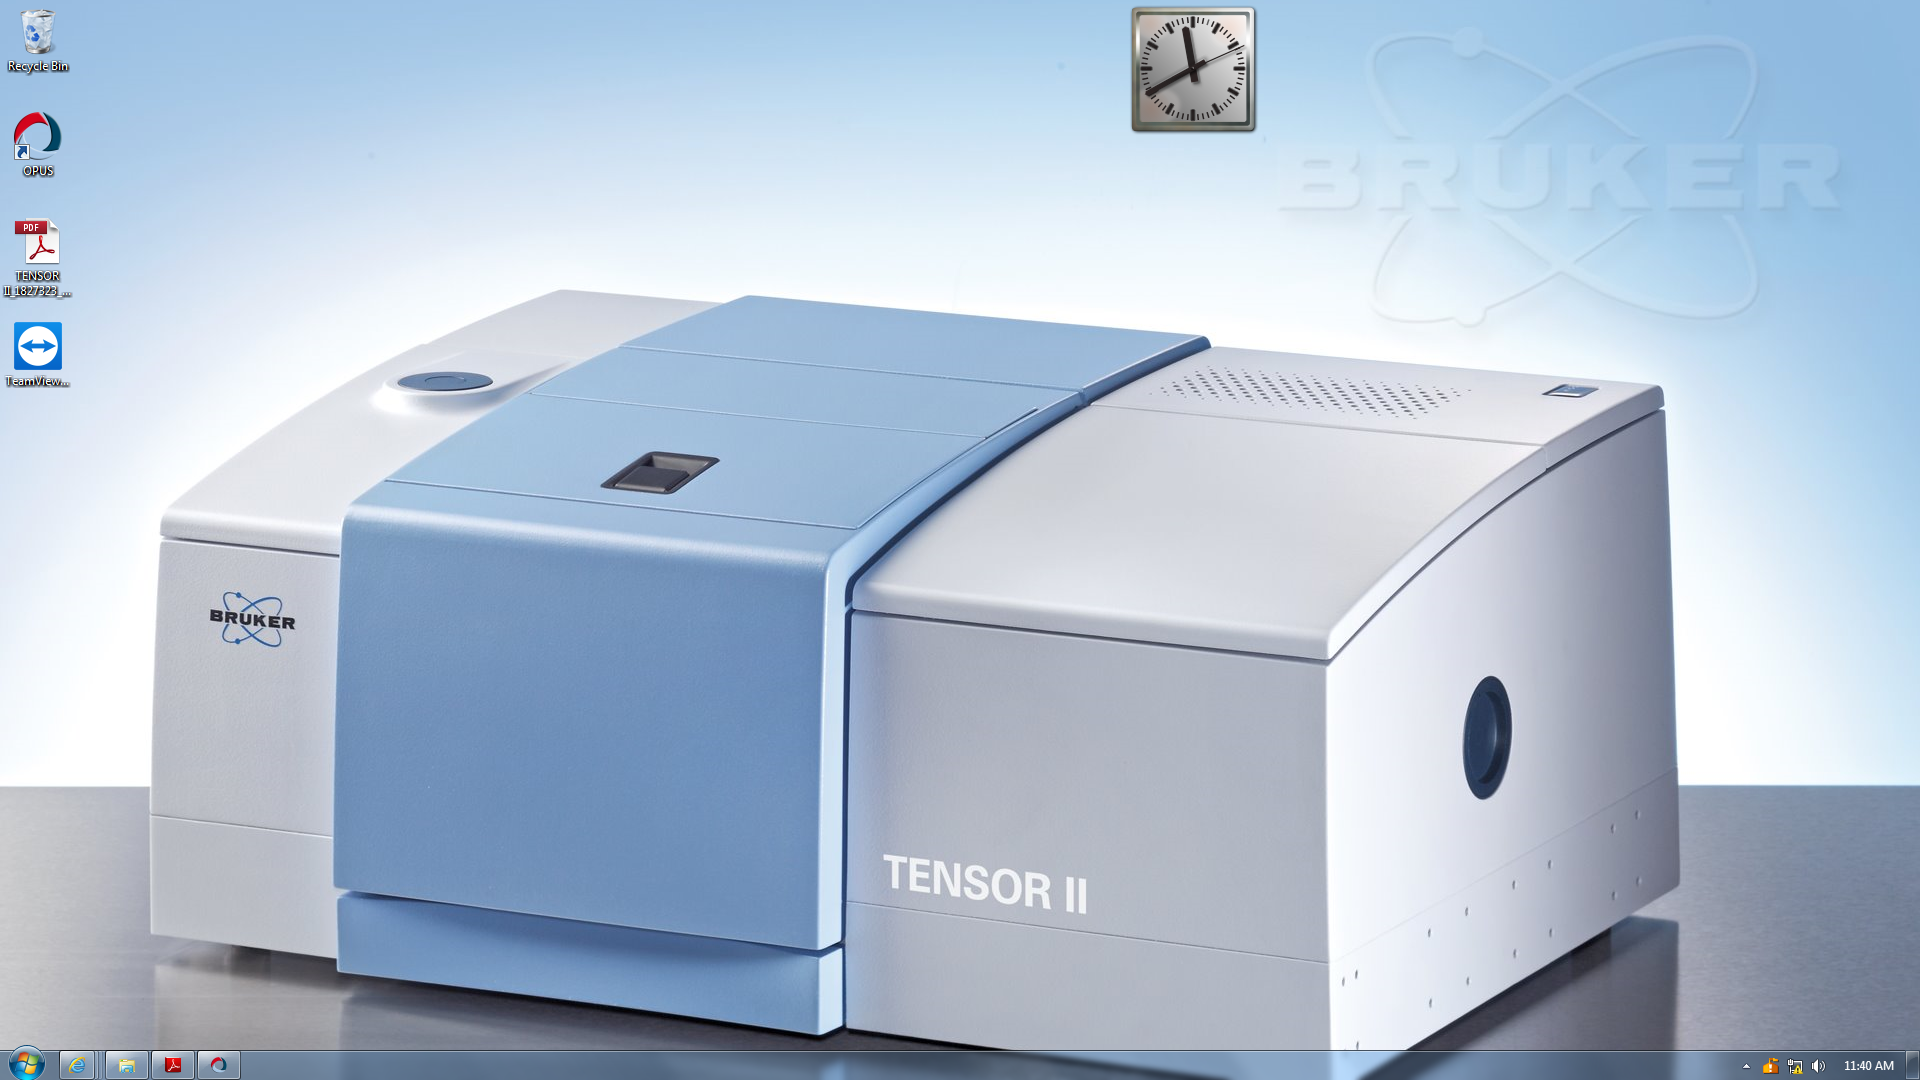
\includegraphics[width=6.5in]{desktop.PNG}
\caption{Desktop.}
\label{desktopicon}
\end{center}
\end{figure}

    \item Log in with the following credentials and workspace (see Figure \ref{OPUS_Login}):
    \begin{itemize}
        \item User ID: \verb|Administrator|
        \item Password: \verb|OPUS|
        \item Assigned workspace: \verb|EPA.ows|
\begin{figure}[htb]
\begin{center}
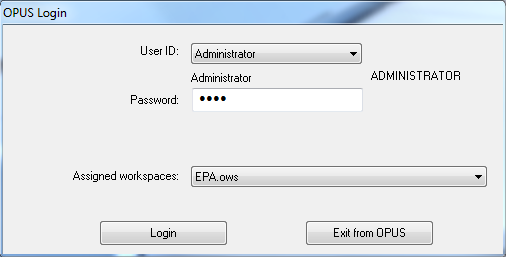
\includegraphics[]{OPUS_Login.PNG}
\caption{OPUS Login.}
\label{OPUS_Login}
\end{center}
\end{figure}

    \end{itemize}
    \item Allow the software to run through all the system checks. The status circle in the bottom right corner of the software will be green if the system checks are all OK (Figure \ref{EPA_ows}). For example, the status circle will be red if the liquid nitrogen level in the detector's dewar is too low. Click the status circle to bring up a diagnostics window that will show which system checks need attention (Figure \ref{OPUSdiagnostics}).
\begin{figure}[htb]
    \centering
    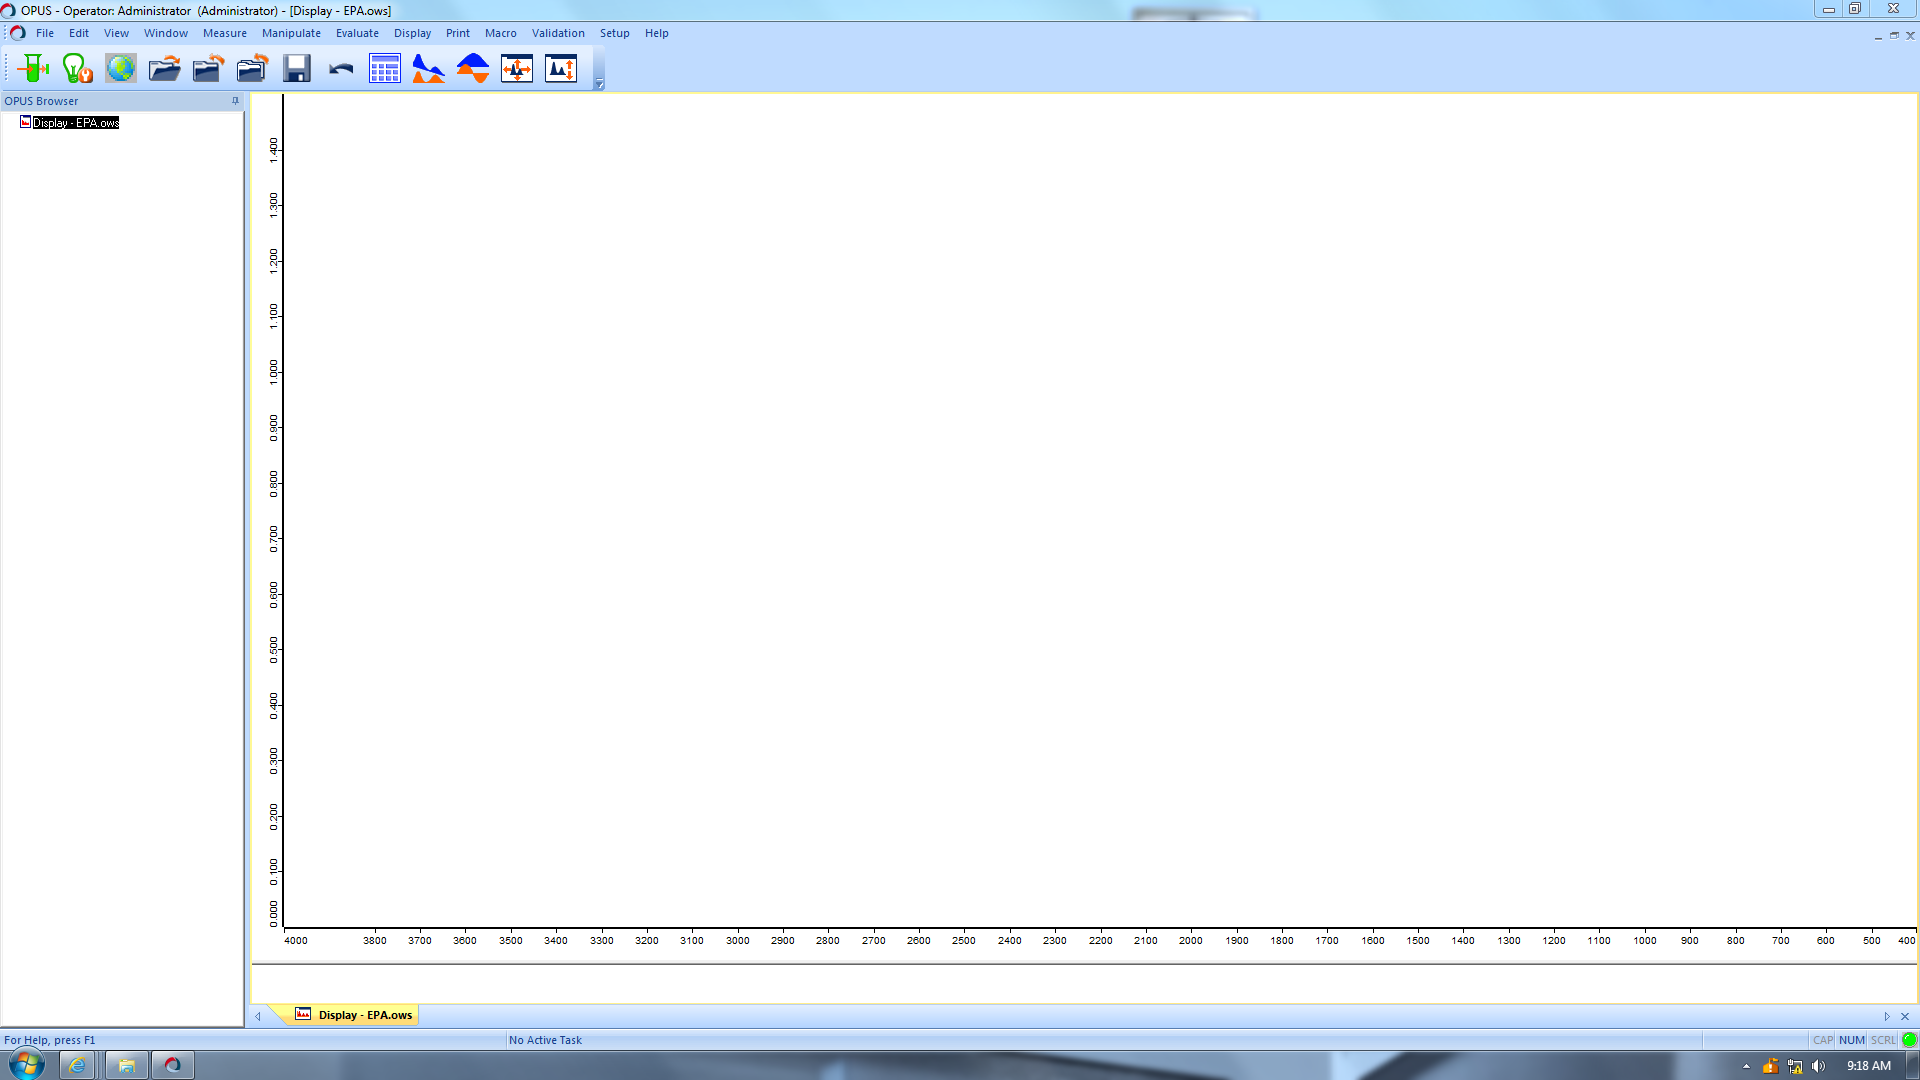
\includegraphics[width=6.5in]{EPA_ows_green.PNG}
    \caption{Starting screen for the OPUS software. The status circle in the bottom right corner should be green. If the status circle is red, click it to open a diagnostics window.}
    \label{EPA_ows}
\end{figure}

\begin{figure}[htb]
\begin{center}
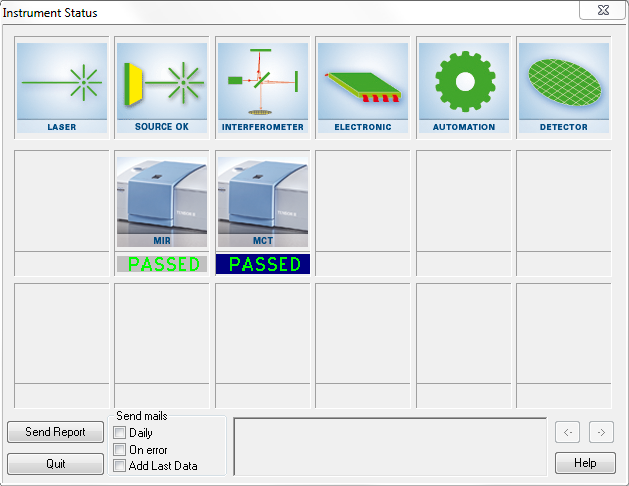
\includegraphics[width=6.5in]{diagnostics.PNG}
\caption{The OPUS diagnostics window for the TENSOR II FT-IR showing all instruments statuses and system checks OK.}
\label{OPUSdiagnostics}
\end{center}
\end{figure}
    \item If the OPUS system checks do not pass, open the diagnostics window by clicking the status circle in the bottom right corner of the OPUS software screen. Follow the TENSOR II user manual to troubleshoot each issue. Common failures include not filling the liquid nitrogen dewar on the detector, or an expired performance test. More details on the instrument tests are available in Section \ref{sec:QC} Quality Control on page \pageref{sec:QC}.
    \end{enumerate}

\subsection{Taking a routine measurement}
\label{subsec:measurement}
\begin{enumerate}
    \item List the desired sample names in the text file \verb|Sample_list.txt|. Note that this can be any text file where each line is the desired name for each sample to be measured. \\ \colorbox{orange}{CAUTION:} The last line will be ignored by the measurement routine, so be sure to terminate the .txt file with a final filler line such as ``\verb|sample_x|” so that the last sample is included in measurements.
    \item Save and close the notepad.
    \item To start a routine measurement, click the ``Background/Filter Scan" icon, which looks like a globe of planet earth in the toolbar at the top left of the workspace (see again Figure \ref{EPA_ows}).
    \item In the Measurement Parameters window (Figure \ref{routineparameters}), check that the following fields are filled out:
    \begin{itemize}
        \item XPM File:
        \begin{itemize}
            \item Path: \verb|C:\Users\Public\Documents\Bruker\OPUS_7.5.18\XPM\|
            \item Name: \verb|BrukerXPM2.xpm|
        \end{itemize}
        \item Force to acquire new background in \textbf{60} minutes
        \item Wait time before acquiring background \textbf{0} seconds
        \item Wait time before measuring sample \textbf{180} seconds
        \item Text File Containing Sample Names
        \begin{itemize}
            \item Path: \verb|C:\Temp|
            \item Name: \verb|Sample_list.txt|
        \end{itemize}
    \end{itemize}
    Entering 180 seconds into the field ``Wait time before measuring sample" sets up the sample compartment to purge for 180 seconds, or for 3 minutes before starting each measurement.
\begin{figure}[htp]
    \centering
    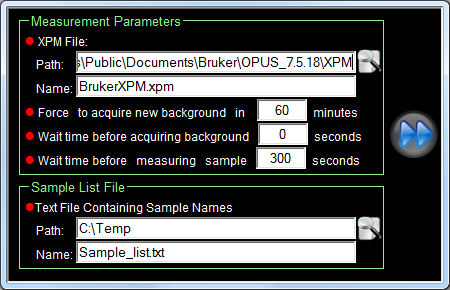
\includegraphics{RoutineMeasurement.PNG}
    \caption{Parameters for routine measurement.}
    \label{routineparameters}
\end{figure}
    \item Proceed by clicking the blue arrows. 
%    \item Follow on-screen prompts for acquiring background and samples.
    \item The system will prompt the user to measure an empty background as a reference. Make sure the sample chamber is empty and closed, and then click OK to proceed.
    \item Wait for the measurement to be taken. %The measurement parameters entered in previous steps will instruct the instrument to wait 3 minutes for the sample compartment to purge, and then take 512 scans.
    \item When the measurement is complete, the system will prompt you to insert a sample. First check the sample name and the corresponding filter label, then place the matching filter into the sample holder. The collection side of the filter should face the IR light source beam. Close the sample holder fully, and then click OK to proceed. \\ \colorbox{orange}{CAUTION:} The system will initiate the 180-second wait time for the sample measurement as soon as the user clicks OK, so to ensure a consistent purge time between each sample, be sure to only click OK after the sample filter is slotted into place inside the sample holder and the cover is fully shut.
    \item Repeat steps 7 and 8 until the measurements for all the samples in the \verb|Sample_list.txt| are complete. If the background measurement expires (which is scheduled to occur after 60 minutes of measurements), re-measure the empty chamber as needed.
    \item Locate the measurement files in the directory \verb|C:\FTIR_Data|. There will be two files saved for each sample measurement: a spreadsheet ``\verb|.csv|" and an OPUS file ``\verb|.0|". If the \verb|Sample_list.txt| included duplicate sample names, the second duplicate will have file extension ``.1", the third will have file extension ``.2", etc. The background measurement has automatically been subtracted from each sample measurement.
    \item Move all the sample files (both \verb|.csv| and OPUS files) into a folder labeled \verb|[yymmdd-xx]|, where \verb|xx| is the experiment number for that day. For example, the third set of measurements taken on April 4, 2018 would be in the folder labeled ``\verb|180404-03|" (see Figure \ref{screenshotfiles}).
\end{enumerate}

\begin{figure}[htb]
\begin{center}
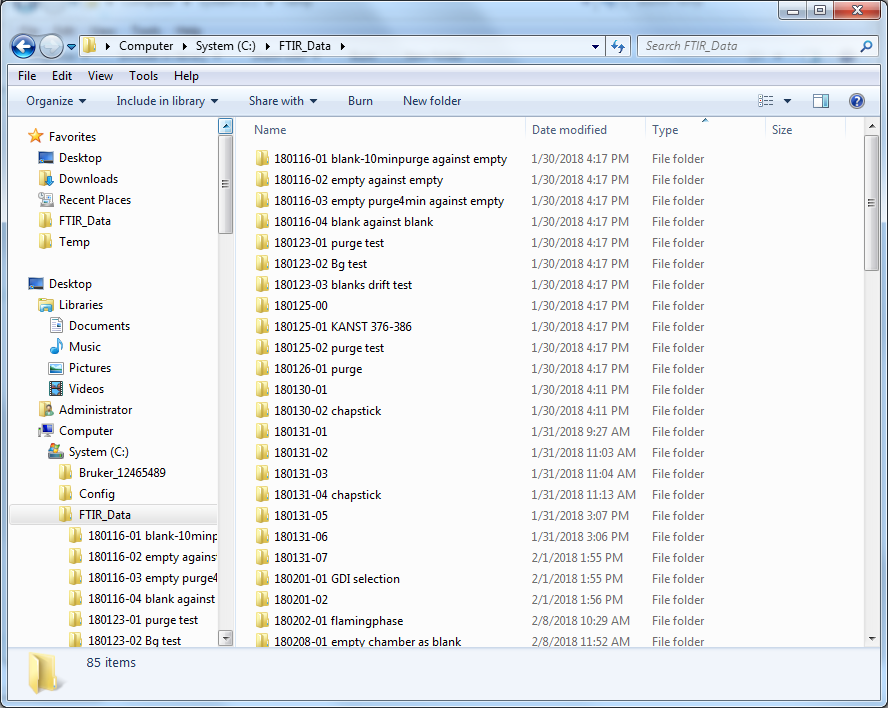
\includegraphics[width=6.5in]{data.PNG}
\caption{File directory for FT-IR measurements.}
\label{screenshotfiles}
\end{center}
\end{figure}

\subsection{Taking screenshots in the OPUS software}
To take screenshots of spectra in the OPUS software, select the OPUS window displaying the desired spectra and axes. Press Ctrl+C. Open Paint and press Ctrl+V. Save as a \verb|.png|.

\subsection{Shutting down}
\begin{enumerate}
    \item Save data as necessary as described in Steps 10-11 in Subsection \ref{subsec:measurement} on page \pageref{subsec:measurement}.
    \item Close the OPUS software and any other associated open program by clicking the x in the top right-hand corner or clicking on the File menu and selecting Exit.
    \item \textbf{Do not turn off the instrument.} As described in the TENSOR II User Manual, the instrument should be left on overnights and over the weekends. The TENSOR II spectrometer should only be switched off in case of a long time of nonuse.
\end{enumerate}

\subsection{Data description and calculations}
The OPUS software saves both a \verb|.0| and a \verb|.csv| file for each spectrum taken (see Figure \ref{screenshotfiles}). Data can be viewed directly in the OPUS software by importing \verb|.0| files.

The \verb|.csv| data file consists of two columns of wavenumber and relative absorbance data. 

\subsection{Data analysis}
FT-IR spectra of particle matter collected on Teflon membrane filters will be analyzed for functional group composition and for calibration of various chemical entities. A baseline correction is required prior to performing peak-fitting for functional group analysis. Typically smoothing splines are used to perform the baseline correction \cite{Kuzmiakova1}. Peak-fitting for functional group characterization is described exhaustively in Takahama et al. 2013 \cite{Satoshi1}; similar methods will be applied here. Calibration for determination of a variety of chemical entities, e.g. OC-EC, will be performed using a multivariate regression analysis as described earlier \cite{Reggente1}. Baseline correction may also be performed prior to using FT-IR spectra for calibration. On-line chemometric tools developed for processing of FT-IR spectra are available at \url{http://airspec.epfl.ch/}.

Table \ref{tab:bonds} provides functional group characterization by wavenumbers.

\begin{table}[H]
    \centering
    \begin{tabular}{l r}
         \textbf{Bond type} & \textbf{Corresponding wavenumbers ($cm^{-1}$)}\cite{Satoshi1} \\
         carbonyl $CO$ & 1720--1714 \\
         amine $NH$ & 1630--1620 \\
         carboxylic $COH$ & 3500--2400 \\
         ammonium $NH$ & 3400--2700 \\
         alcohol $COH$ & 3500--3377, 3371--3203 \\
         alkane $CH$ & 2932--2921, 2886--2882, 2855--2849, 2805--2800 \\
         alkene $CH$ & 3050 \\
         aromatic $CH$ & 2980 \\
    \end{tabular}
    \caption{Target functional group bond types and their associated FT-IR spectral wavenumber(s) or wavenumber range(s).}
    \label{tab:bonds}
\end{table}

